\section{Firewall, Intrusion Detection Systems (IDS) e Architetture di Sicurezza}

% ===========================================================
\subsection{Introduzione ai Firewall e Obiettivi di Design}
% ===========================================================

Nel moderno panorama di cybersecurity, il
\textbf{firewall rappresenta il pilastro fondamentale della difesa
perimetrale}. Agendo come uno strato di protezione strategico, il suo
compito primario è isolare i sistemi interni dalle reti esterne
potenzialmente ostili, stabilendo un collegamento controllato tra domini
di fiducia differenti.

% -----------------------------------------------------------
\subsubsection{Definizione e Posizionamento Strategico}
% -----------------------------------------------------------

Il firewall è un dispositivo progettato per fornire un isolamento
controllato tra una rete locale (\textit{``Promised Network''}) e
l'ambiente non fidato di Internet. Secondo il \textit{General Model of
FW}, il dispositivo si interpone come muro fiammeggiante tra la
\textit{``Internal (Protected) Network''} e la \textit{``External
(Untrusted) Network''}. La sua distinzione risponde a obiettivi
strategici precisi: proteggere la rete interna dagli attacchi basati su
Internet e stabilire un punto di saldatura unico (\textbf{Single Choke
Point}). Questo nodo critico funge da punto di monitoraggio
(\textit{Monitoring Junction}) dove le politiche di sicurezza e
l'auditing possono essere imposte centralmente. Frequentemente, il
firewall viene collocato con altre funzioni di rete, come il gateway
VPN, per consolidare il perimetro.

% -----------------------------------------------------------
\subsubsection{Obiettivi di Design}
% -----------------------------------------------------------

Un firewall efficace deve essere progettato seguendo tre criteri imprescindibili:

\begin{itemize}
    \item \textbf{Transito Obbligato}: tutto il traffico, sia in entrata che in uscita, 
    deve passare necessariamente attraverso il firewall. Ciò richiede il blocco fisico di 
    ogni via d'accesso alternativa alla rete locale.
    \item \textbf{Autorizzazione}: solo il traffico esplicitamente ammesso dalla politica di 
    sicurezza locale è autorizzato a transitare. Diverse tipologie di firewall implementano queste 
    politiche con gradi di granularità differenti.
    \item \textbf{Immunità}: il firewall stesso deve essere impenetrabile. Questo obiettivo si 
    raggiunge utilizzando sistemi \textit{hardened} (irrobustiti) e sistemi operativi sicuri 
    (\textit{Secured OS}) standard, spesso basati su linguaggi conservativi.
\end{itemize}

% -----------------------------------------------------------
\subsubsection{Tecniche di Controllo degli Accessi}
% -----------------------------------------------------------

Per garantire l'applicazione rigorosa della politica di sicurezza, si utilizzano quattro modalità di controllo:

\begin{enumerate}
    \item \textbf{Service Control (Controllo dei Servizi)}: determina quali servizi (es. HTTP, SFTP) sono accessibili.
    \item \textbf{Direction Control (Controllo della Direzione)}: specifica la direzione in cui può essere 
    avviata una richiesta (es. solo dall'interno verso l'esterno).
    \item \textbf{User Control (Controllo dell'Utente)}: regola l'accesso in base all'identità; richiede spesso 
    l'autenticazione per gli utenti esterni.
    \item \textbf{Behavior Control (Controllo del Comportamento)}: monitora come i servizi vengono effettivamente 
    utilizzati (es. filtraggio anti-spam).
\end{enumerate}

% ===========================================================
\subsection{Limitazioni e Confronto tra Approcci: Rule vs Policy}
% ===========================================================

L'evoluzione delle minacce informatiche ha evidenziato la necessità di
passare da sistemi di filtraggio statico a modelli contestuali più
flessibili, poiché i firewall tradizionali presentano \textit{``punti
ciechi''} strutturali.

% -----------------------------------------------------------
\subsubsection{Limitazioni Intrinseche}
% -----------------------------------------------------------

Un firewall non può intercettare attacchi che bypassano il dispositivo, come l'uso di connessioni 
dial-out verso ISP esterni o accessi tramite reti wireless (WLAN) non protette. Inoltre, il firewall 
offre una protezione limitata contro le minacce interne, siano esse azioni dolose di dipendenti 
o l'introduzione involontaria di malware tramite dispositivi infettati fisicamente e poi connessi alla LAN aziendale.

% -----------------------------------------------------------
\subsubsection{Firewall Rule-Based (Basati su Regole)}
% -----------------------------------------------------------

Questi sistemi operano in modo statico: ogni azione deve essere espressamente configurata in 
un file di configurazione per ogni pacchetto. Se non esiste una regola specifica, il sistema non può adattarsi.
Offre in vantaggio una configurazione lineare e intuitiva.

Esempio: \textit{regola che permette il traffico DNS esclusivamente verso un server esterno noto.}

% -----------------------------------------------------------
\subsubsection{Firewall Policy-Based (Basati su Politiche)}
% -----------------------------------------------------------

Questi sistemi offrono una flessibilità superiore, permettendo all'amministratore di definire 
condizioni generali e funzioni specifiche. Un sistema policy-based può gestire dinamicamente 
connessioni verso IP casuali, come richiesto dai protocolli IPsec (AH/ESP). Un esempio di logica 
multidimensionale è:

\begin{quote}
\textit{``Consenti l'accesso al server CRM solo tra le 9:00 e le 18:00, solo se l'antivirus del 
client è aggiornato, l'utente appartiene alla VLAN `Sales' e l'identità è verificata tramite SSO.''}
\end{quote}

I sistemi basati su regole faticano a gestire tale logica per diversi motivi:

\begin{itemize}
    \item \textbf{Vincoli Temporali}: richiedono meccanismi di scheduling complessi.
    \item \textbf{Device Posture}: incapacità di valutare la salute dell'endpoint (AV status).
    \item \textbf{Integrazione Livelli 2--7}: la combinazione di VLAN (L2), IP (L3) e identità (L7) 
    richiede un'awareness che i sistemi statici non possiedono.
    \item \textbf{Integrazione SSO}: impossibilità di verificare lo stato dell'autenticazione unica.
\end{itemize}

I sistemi policy-based superano questi limiti utilizzando attributi del dispositivo, identità, 
orari e consapevolezza applicativa per prendere decisioni adattive.

% ===========================================================
\subsection{Tipologie Tecniche di Firewall e Architetture DMZ}
% ===========================================================

La classificazione dei firewall si basa sul livello di ispezione dei protocolli, con un costante 
trade-off tra profondità di analisi e prestazioni. I filtri possono essere \textbf{positivi} 
(ammettono solo ciò che è esplicitamente elencato) o \textbf{negativi} (negano solo ciò che è proibito).

% -----------------------------------------------------------
\subsubsection{Packet Filtering Firewall e Analisi dei Rule Set}
% -----------------------------------------------------------

Il filtraggio dei pacchetti esamina gli header IP e di trasporto (IP sorgente/destinazione, 
porte, protocollo, interfaccia) per decidere se inoltrare (\textit{forward}), negare 
(\textit{deny}) o modificare (\textit{modify}) il traffico.

Dall'analisi dei set di regole emergono diverse logiche di sicurezza:

\begin{itemize}
    \item \textbf{Set A}: applica una diffidenza specifica; la regola \texttt{BLOCK AA SPIGOT} 
    impedisce ogni comunicazione da un host non fidato (\textit{spigot}), permettendo però il 
    traffico SMTP verso il gateway interno.
    \item \textbf{Set B}: implementa una politica di \textit{default deny} (\texttt{BLOCK * * * *}), 
    che è la pratica più sicura.
    \item \textbf{Set C}: regola permissiva che consente a qualsiasi host interno di connettersi 
    a un server SMTP esterno (porta 25).
    \item \textbf{Set D}: introduce il controllo dei flag TCP. La prima riga permette ai nostri 
    host di inviare pacchetti verso la porta 25 esterna; la seconda riga permette le risposte 
    (ACK) dall'esterno, impedendo che un host esterno inizi una connessione non richiesta.
    \item \textbf{Set E}: gestisce il traffico verso i ``non servers'': permette le chiamate 
    in uscita, le relative risposte (ACK) e il traffico verso porte superiori a 1024, tipicamente 
    usate per le connessioni effimere dei client.
\end{itemize}

I filtri di pacchetto sono vulnerabili ad attacchi come:
\begin{itemize}
    \item \textbf{IP Address Spoofing} --- Contromisura: controllo dell'interfaccia di ingresso.
    \item \textbf{Source Routing Attacks} --- Contromisura: blocco delle opzioni di source route.
    \item \textbf{Tiny Fragment Attacks}, dove l'attaccante frammenta il pacchetto per nascondere 
    l'header di trasporto --- Contromisura: verifica della dimensione minima del pacchetto.
\end{itemize}

% -----------------------------------------------------------
\subsubsection{Firewall Avanzati: Stateful, Application e Circuit-Level}
% -----------------------------------------------------------

\begin{enumerate}
    \item \textbf{Stateful Inspection Firewall}: questi sistemi tracciano lo stato delle connessioni 
    TCP in una tabella dedicata (stati \texttt{ESTABLISHED}, \texttt{RELATED}). Sono in grado di 
    prevenire il session hijacking tracciando i numeri di sequenza. Un aspetto pedagogico importante 
    è la gestione dei protocolli multi-canale come SIP: il firewall riconosce che il traffico 
    audio/video RTP è ``correlato'' all'interno della sessione di segnalazione e apre dinamicamente 
    le porte necessarie.
    \item \textbf{Application-Level Gateway (Proxy)}: agisce come un relay completo. L'utente si connette 
    al proxy, si autentica e il proxy stabilisce una nuova connessione verso l'esterno. Offre un logging 
    più dettagliato ma supporta solo applicazioni specifiche.
    \item \textbf{Circuit-Level Gateway}: sfrutta la connessione TCP in due segmenti (interno ed esterno) 
    senza ispezionare il payload. Viene usato quando l'amministratore si fida degli utenti interni per 
    le connessioni outbound.
\end{enumerate}

\begin{figure}[H]
    \centering
    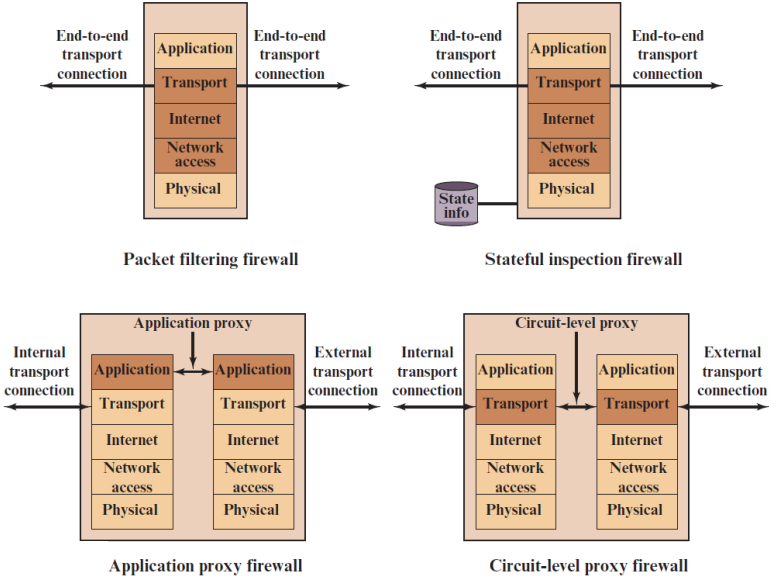
\includegraphics[width=0.8\textwidth]{img/firewall.png}
\end{figure}

% -----------------------------------------------------------
\subsubsection{Architettura DMZ (Demilitarized Zone)}
% -----------------------------------------------------------

La rete viene segmentata per proteggere i servizi esposti. Il traffico da Internet attraversa 
prima un \textit{Boundary Router}, poi un \textit{External Firewall} che scherma la DMZ 
(Web, Email, DNS). Un \textit{Internal Firewall} protegge infine la \textit{``Internal Protected Network''} 
(App/DB server, workstation).

L'Internal FW ha compiti critici: applica filtri più stringenti e fornisce una protezione bidirezionale. 
Protegge il core aziendale da attacchi provenienti da macchine DMZ compromesse (evitando la propagazione 
di worm, rootkit o bot) e, al contempo, scherma la DMZ da potenziali minacce interne.

% ===========================================================
\subsection{Architettura Zero Trust (ZTA)}
% ===========================================================

Il modello tradizionale \textit{``Castle-and-Moat''} (castello con fossato), basato sulla fiducia 
implicita per chiunque si trovi all'interno del perimetro, è oggi superato. In tale modello, una 
volta violato il perimetro, l'attaccante ha libertà di movimento laterale.

% -----------------------------------------------------------
\subsubsection{Principi e Benefici della Zero Trust}
% -----------------------------------------------------------

Il dogma centrale è \textbf{``Never Trust, Always Verify''}. Nessuna entità è fidata per default, 
a prescindere dalla posizione logica o fisica. Questo approccio è necessario nell'era del cloud, 
ove i dati sono distribuiti e il perimetro è fluido. I benefici includono la conformità normativa 
(GDPR), la protezione dei dati tramite crittografia e una sicurezza robusta per il lavoro remoto.

% -----------------------------------------------------------
\subsubsection{Pilastri e Concetti Operativi}
% -----------------------------------------------------------

I \textit{Zero Trust Pillars} identificano: Identità, Dispositivi, Rete, Infrastruttura, 
Applicazioni, Visibilità, Analisi e Automazione. I concetti chiave includono:

\begin{itemize}
    \item \textbf{Least Privilege (Minimo Privilegio)}: accesso limitato
    allo stretto necessario. Le VPN sono spesso inadatte perché
    concedono visibilità sull'intera rete.
    \item \textbf{Microsegmentazione}: divisione della rete in zone minuscole e isolate.
    \item \textbf{Prevenzione del Movimento Laterale}: grazie alla
    ri-autenticazione periodica e al timeout delle sessioni, un
    attaccante non può spostarsi tra segmenti. Se un account viene
    compromesso, viene isolato (quarantena).
    \item \textbf{Best Practices}: uso di MFA basata su chiavi hardware
    (token invece di OTP software), integrazione della Threat
    Intelligence e monitoraggio continuo dell'integrità dei dispositivi.
    È fondamentale non indurre gli utenti a eludere la sicurezza con
    misure eccessivamente oppressive.
\end{itemize}

% ===========================================================
\subsection{Intrusion Detection Systems (IDS) e Metriche di Performance}
% ===========================================================

Mentre il firewall agisce in modo preventivo, l'IDS monitora gli eventi
per identificare i tentativi di violazione delle proprietà CIA
(Confidentiality, Integrity, Availability).

% -----------------------------------------------------------
\subsubsection{Architettura e Posizionamento}
% -----------------------------------------------------------

L'IDS è composto da \textbf{sensori} (raccolta pacchetti, log, system
call), \textbf{analizzatori} (motore decisionale) e \textbf{user
interface}. In un'architettura di rete, i NIDS (Network IDS) vengono
posizionati strategicamente in quattro punti:

\begin{enumerate}
    \item \textbf{1 (Esterna)}: per rilevare tentativi di attacco diretti prima del firewall.
    \item \textbf{2 (DMZ)}: per monitorare il traffico verso i servizi esposti.
    \item \textbf{3 (Core Network)}: per proteggere i server critici e i dati sensibili.
    \item \textbf{4 (Workstation)}: per identificare minacce interne o traffico laterale tra client.
\end{enumerate}

\begin{figure}[H]
\centering
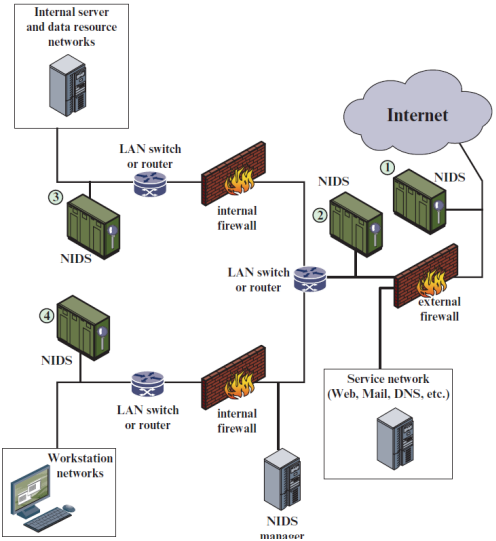
\includegraphics[width=0.5\textwidth]{img/IDS.png}
\end{figure}

% -----------------------------------------------------------
\subsubsection{Approcci al Rilevamento}
% -----------------------------------------------------------

\begin{itemize}
    \item \textbf{Misuse Detection}: basato su firme note (string, port,
    o header condition signatures). Offre alte prestazioni e pochi falsi
    positivi.
    \item \textbf{Anomaly Detection}: basato sulla deviazione dal
    comportamento normale. È fondamentale per gli attacchi zero-day.
    Richiede un approccio probabilistico, spesso supportato dal Machine
    Learning.
\end{itemize}

% -----------------------------------------------------------
\subsubsection{Metriche di Performance e Rigore Matematico}
% -----------------------------------------------------------

L'efficacia viene valutata tramite la \textit{Confusion Matrix}
(Attack/No Attack vs Anomaly/No Anomaly). Le metriche fondamentali sono:

\begin{itemize}
    \item \textbf{Accuracy (Accuratezza)}:
    \[
        A = \frac{TP + TN}{TP + TN + FP + FN}
    \]
    \item \textbf{Precision (Precisione)}:
    \[
        P = \frac{TP}{TP + FP}
    \]
    \item \textbf{Recall (Richiamo / Sensibilità)}:
    \[
        R = \frac{TP}{TP + FN}
    \]
    \item \textbf{F-Score} (penalizza valori estremi):
    \[
        F = \frac{2 \cdot P \cdot R}{P + R} = \frac{2TP}{2TP + FP + FN}
    \]
\end{itemize}

L'analisi avanzata utilizza la \textbf{curva ROC}
(\textit{Receiver Operating Characteristic}) che mette in relazione il
TPR (\textit{Hits / (Hits + Misses)}) e il FPR (\textit{False Alarms /
(False Alarms + Correct Rejections)}):
\[
    FPR = \frac{FP}{FP + TN}
\]

L'\textbf{AUC} (\textit{Area Under Curve}) rappresenta la probabilità
che un campione positivo scelto casualmente riceva un punteggio
superiore a uno negativo. In questo ambito, la
\textbf{explainability} (spiegabilità) delle decisioni di ML è cruciale
per permettere agli amministratori di comprendere il ``perché'' di un
allarme.

% -----------------------------------------------------------
\subsubsection{Acquisizione e Feature Engineering}
% -----------------------------------------------------------

Nell'anomaly detection basata sui dati, il \textbf{feature engineering}
è vitale: è necessario selezionare caratteristiche significative,
eliminando quelle correlate tra loro o non rilevanti per l'analisi. Per
stabilire soglie di allarme robuste, si preferisce l'uso della
\textbf{MAD} (\textit{Median Absolute Deviation}) rispetto alla semplice
media, poiché la MAD è significativamente più robusta agli outlier
presenti nei dataset di rete reali.

% ===========================================================
\subsection{Attacchi Distributed Denial of Service (DDoS)}
% ===========================================================

Gli attacchi DDoS mirano a esaurire le risorse di calcolo (es.
limitando le connessioni TCP) o di trasmissione (inondando la banda con
ICMP/UDP), compromettendo la disponibilità del servizio.

% -----------------------------------------------------------
\subsubsection{Procedure di Scansione e Reclutamento}
% -----------------------------------------------------------

Gli attacchi identificano vulnerabilità per creare macchine ``zombie'' tramite quattro tecniche di scansione:

\begin{enumerate}
    \item \textbf{Random Probing}: ricerca casuale di indirizzi IP (facile da rilevare se troppo rapida).
    \item \textbf{Hit List}: scansione di una lista predefinita di host potenzialmente vulnerabili.
    \item \textbf{Topologica}: utilizza le informazioni residenti
    sull'host già infetto (es. rubriche o connessioni locali) per
    propagarsi.
    \item \textbf{Local Subnet}: ricerca di target dietro lo stesso firewall della macchina infetta.
\end{enumerate}

% -----------------------------------------------------------
\subsubsection{Architetture di Attacco e Strategie di Difesa}
% -----------------------------------------------------------

\begin{itemize}
    \item \textbf{Direct Attack}: l'attaccante comanda gli zombie primari, che istruiscono 
    gli agenti a inondare direttamente la vittima.

    \begin{figure}[H]
    \centering
    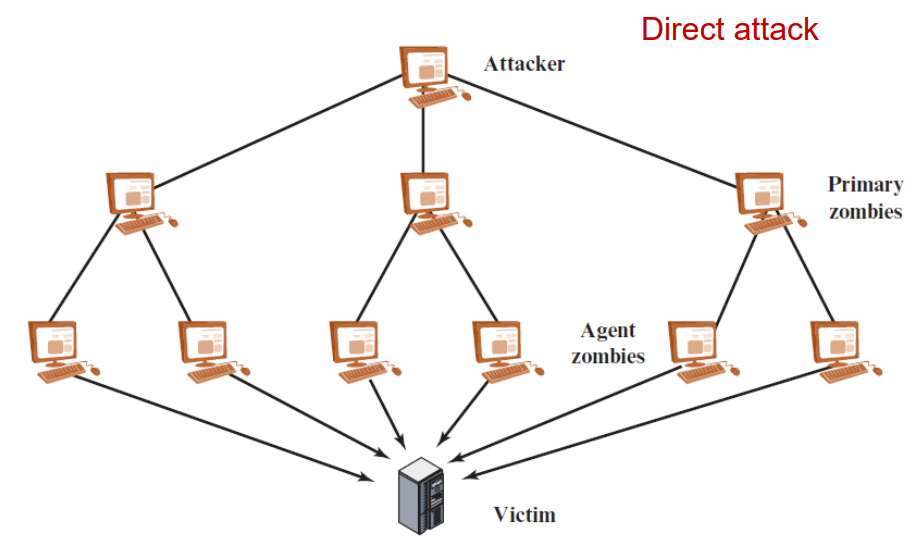
\includegraphics[width=0.8\textwidth]{img/directAttack.png}
    \end{figure}

    \item \textbf{Reflector Attack}: gli agenti inviano richieste (spesso pacchetti SYN) 
    a macchine riflettore innocue, falsificando l'IP sorgente con quello della vittima. 
    I riflettori rispondono alla vittima, inondandola e nascondendo l'identità degli agenti.

    \begin{figure}[H]
    \centering
    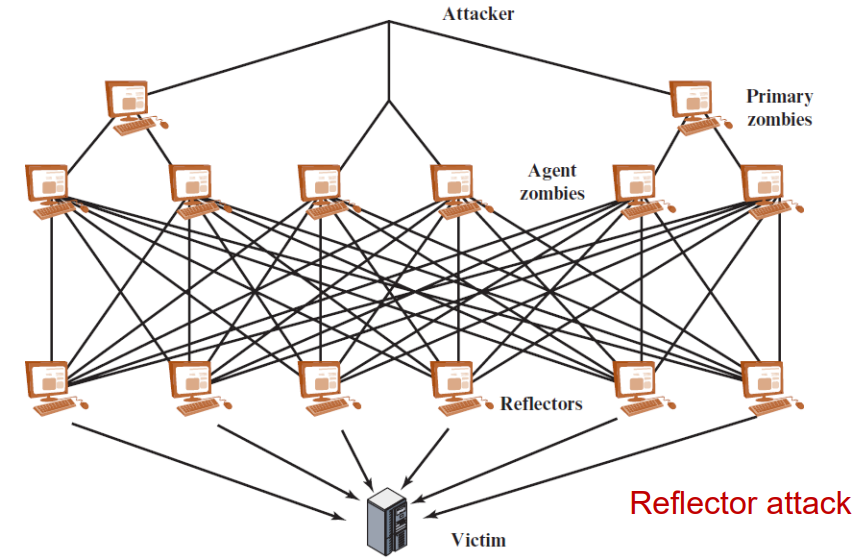
\includegraphics[width=0.8\textwidth]{img/reflectorAttack.png}
    \end{figure}

\end{itemize}

Le contromisure si articolano in tre fasi:

\begin{enumerate}
    \item \textbf{Prevenzione}: patching e policy rigorose prima dell'evento.
    \item \textbf{Rilevamento e Filtraggio}: risposta immediata durante l'attacco tramite monitoraggio continuo.
    \item \textbf{Tracciamento}: identificazione post-attacco della
    sorgente, operazione complessa volta a prevenire futuri incidenti.
\end{enumerate}

In sintesi, solo un'integrazione coerente tra firewall, IDS e una
filosofia \textbf{Zero Trust} può garantire una postura di sicurezza
resiliente contro le minacce distribuite e sofisticate di oggi.

\begin{figure}[H]
\centering
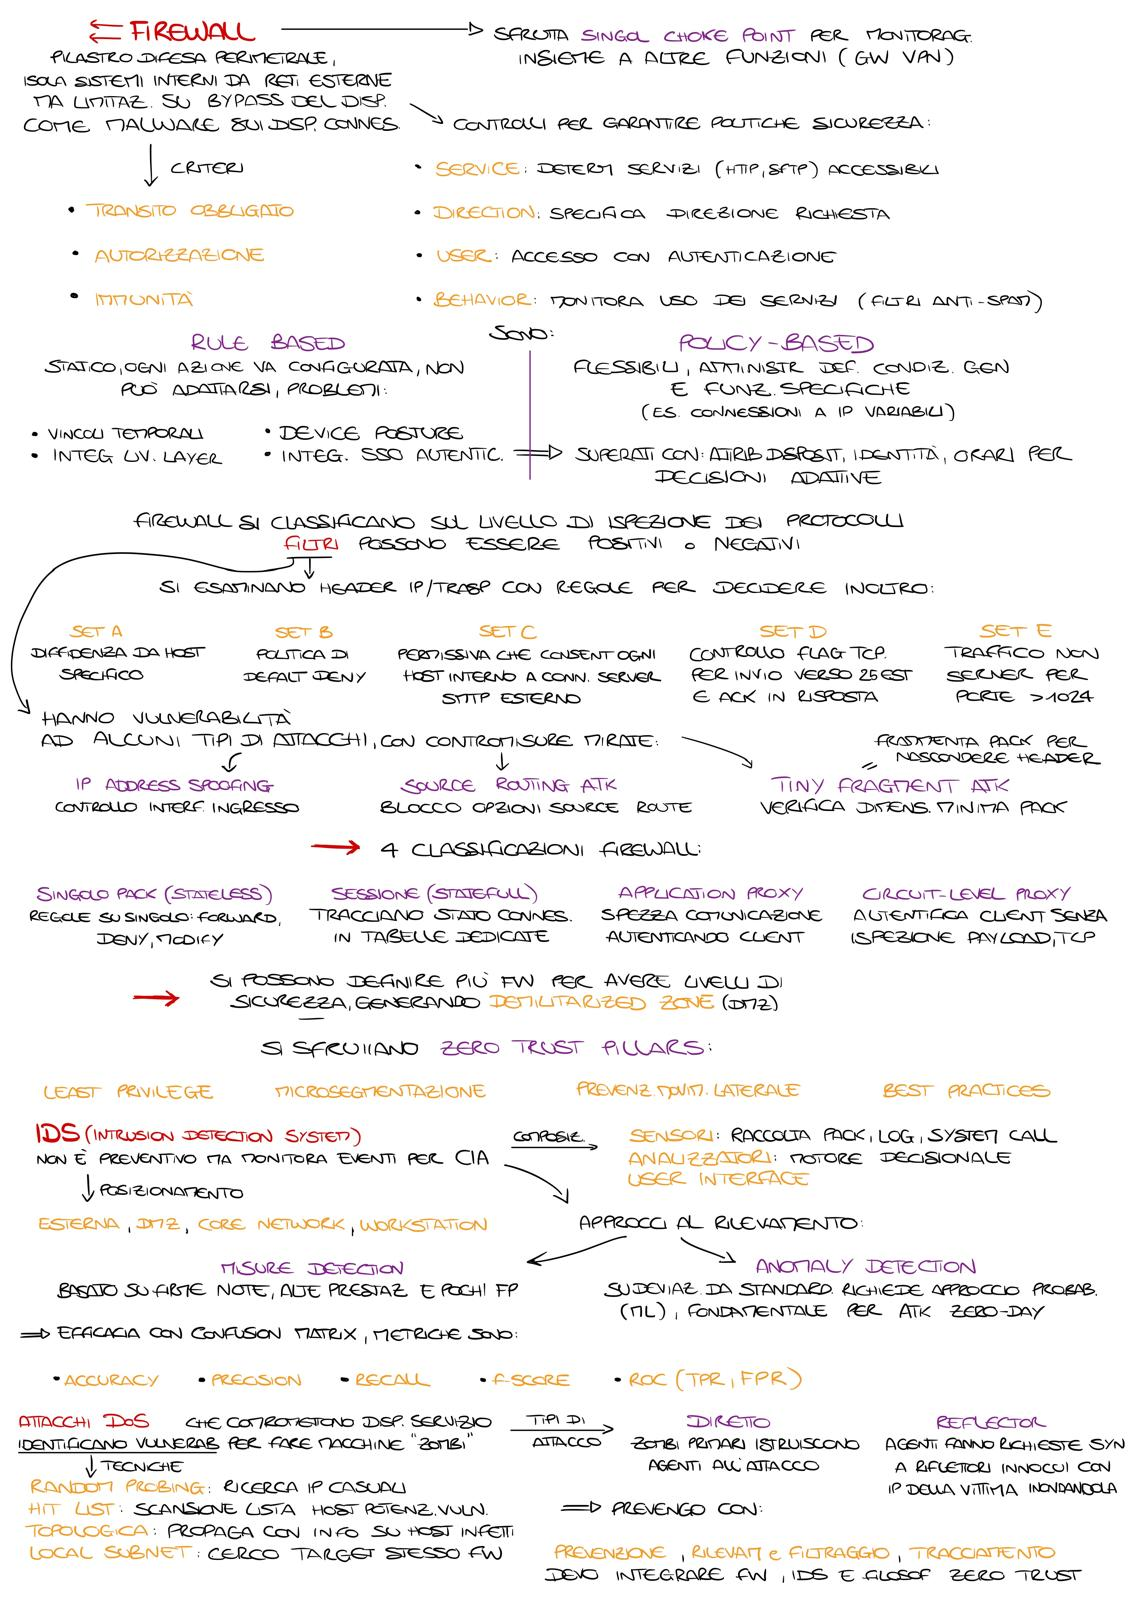
\includegraphics[width=1\textwidth]{img/4.png}
\end{figure}
